\section{Selection of the cross section}

The cross section selection process for this study was based to three key criteria 

\begin{itemize}
	\item The cross section should have a bluff front face with sharp upstream corners for the flow to separate at the leading edges;
	
	\item As the proximity of shear layers to the body plays a vital role in creating \cy\ \citep{Parkinson1989}, the cross section should have a basic level of streamlining.
	
	\item The cross section should consist of a geometric profile in the afterbody, to inhibit or delay the shear layer reattachment.   
\end{itemize}


The square cross section which has been widely used in galloping studies satisfies the first two selection criteria. Thus, a modification to the square cross section was done in order to meet the third criterion. Thus, in order to inhibit the shear layer reattachment, the top and bottom sides of the trailing edges of the square were tapered off and a hybrid cross section of a rectangle and a triangle (illustrated in figure \ref{fig:hybrid_section}), i.e, a pentagon was produced.

\begin{figure}
\setlength{\unitlength}{\textwidth}

  \begin{picture}(1,0.23)(0,0.74)
    
  \put(0.2,0.76){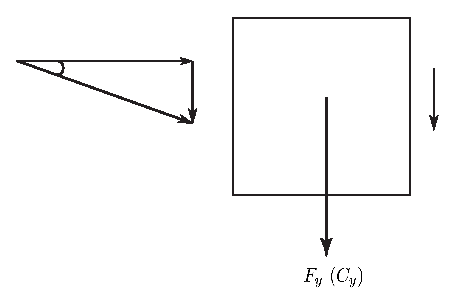
\includegraphics[width=0.5\unitlength]{../FnP/gnuplot/setup-1.eps}}         
      
      
   
 	\put(0.315,0.93){$U$}
 	\put(0.3,0.84){$U_i$}
    \put(0.42,0.88){$\dot{y}$}
    \put(0.28,0.895){ $\theta$}
    \put(0.7,0.87){\small $(+)$}
      	

 	
 	 

     

  \end{picture}

 \caption{Induced angle of attack on the square prism due to the resultant of free-stream velocity of the fluid and transverse velocity of the body.}
    \label{fig:setup_1}
\end{figure}

The inhibition of the shear layer can be varied systematically by varying one parameter, \ratio; which was an advantage of this cross section. The ratio $\ratio$ was varied from 1 to zero in increments of 0.25 where 1 is the square cross section and 0 is an isosceles triangle. 


\section{Static body results}


\begin{table}[ht]

\begin{center}
\setlength{\unitlength}{\textwidth}

\begin{tabular}{c c c c c} % centered columns (4 columns)
\hline\hline %inserts double horizontal lines
\\[0.2ex]
Case & $a_1$ & $a_3$ & $a_5$ & $a_7$ \\ [0.8ex] % inserts table 
%heading
\hline 
\\[0.8ex]% inserts single horizontal line
Re=200 & 2.32 & 197.8 & 4301.7 & 30311.9 \\[0.8ex]% inserting body of the table
Re=22300 & 2.69 & 168 & 1670 & 59900 \\ [1ex] % [1ex] adds vertical space
\hline %inserts single line
\end{tabular}

\caption{Coefficient values used in the 7th order interpolation polynomial for high ($Re=22300$) and low ($Re=200$) Reynolds numbers. These data are used as input data to calculate the right-hand side of Eq. \ref{final_equation_motion} throughout this study.}
 
\label{table:cy-coefficients} % is used to refer this table in the text
\end{center}
\end{table}



Stationary time averaged $C_y$ results were obtained for cross sections where $\ratio=$ $1$, $0.75$ ,$0.5$, $0.25$ and $0$ using DNS at $\reynoldsnumber=200$. Table \ref{table:cy-coefficients-hybrid} shows the coefficients of the $7^{th}$ order curve fitting for each cross section. To achieve a better fit, piecewise interpolation using multiple $7th$ order polynomials were incorporated for a single cross section, giving more importance to accurately fitting the positive portion of the $C_{y}$ curve; as the power transfer from the fluid to the body only occurs in this region.

\begin{figure}
  \setlength{\unitlength}{\textwidth}

  \begin{picture}(1,0.75)(0,0)
    % % %90
      % % % Parkinson Data 
      \put(0.035,0.5){\includegraphics[width=0.5\unitlength]{./FnP/lift_curve_sq.eps}}
      \put(0.495,0.5){\includegraphics[width=0.5\unitlength]{./FnP/lift_curve_075.eps}}
      \put(0.035,0.27){\includegraphics[width=0.5\unitlength]{./FnP/lift_curve_05.eps}}
      \put(0.495,0.27){\includegraphics[width=0.5\unitlength]{./FnP/lift_curve_025.eps}}
      \put(0.3,0.0){\includegraphics[width=0.5\unitlength]{./FnP/lift_curve_tri.eps}}
      
      
   
      
      
%      \put(0.23,0.00){ $\displaystyle\frac{c}{\rho\mathcal{A}U}$}
%      \put(0.73,0.00){ $\displaystyle\frac{c}{\rho\mathcal{A}U}$}

      \put(0.3,0.26){$\theta$}
      \put(0.76,0.26){$\theta$}
      \put(0.56,-0.01){$\theta$}
      
      \put(0.01,0.405){$\displaystyle C_y$}
       \put(0.01,0.65){$\displaystyle C_y$}
      \put(0.3,0.14){$\displaystyle C_y$}
      
      \put(0.106,0.705){\small(a)}
      \put(0.565,0.705){\small(b)}
      \put(0.106,0.475){\small(c)}
      \put(0.565,0.475){\small(d)}
      \put(0.37,0.207){\small(e)}
      

  \end{picture}

  \caption{Induced lift coefficient $C_y$ at different angles for selected cross sections. Data presented for cross sections, (a) square, (b) $\ratio=0.75$, (c) $\ratio=0.5$, (d) $\ratio=0.25$ and (e) triangle.}
  \label{fig:lift_curves}
\end{figure} 

The $C_y$ vs. $\theta$ curves in figure \ref{fig:lift_curves-hybrid} show the resultant of the piecewise curve-fits obtained for each cross section. A shift of the peak value of \cy\ to the right can be observed as the \ratio decreases therefore, the peak \cy\ occurs at higher induced angles. The overall trends of this behaviour agrees with trends of \citet{Luo1994} where the peak \cy\ value was shifted to higher induced angles when reattachment was delayed on a trapezoidal body. The peak value of \cy\ occurs at high induced velocities as \ratio\ is decreased because $\theta$ is proportional to the transverse velocity of the body via $\tan{\theta}=\frac{\dot{y}}{U}$. Thus, these bodies with a short straight section, or small \ratio, satisfy one of the three conditions required to optimize the power transfer. 

A negative region could be observed on the \cy vs. $\theta$ curves  where $\ratio\leq0.25$. In this region \cy\ decreases as $\theta$ is increased and the increases after reaching a minimum, non-zero value of $\theta$. The presence of this region indicates an unfavourable power transfer, i.e. power transferred from body to the fluid as the direction of the force and velocity vectors are out of phase. This implies that at low induced angles (when the $\dot{y}$ is low), power transfer is from the body to the fluid and as the transverse velocity increases power transfers from fluid to the body. Thus, it means that the direction of power transfer can be different at different points in a particular oscillation cycle, which will be further discussed in section \hilight{Section}. 



 \section{QSS Mean power output}
 \label{sec:mean power}
 
  
 % !TeX spellcheck = en_GB
\begin{figure}[!htb]
  \setlength{\unitlength}{\textwidth}

        \begin{picture}(1,0.4)(-0.02,0)

 
      
      \put(0.08,0.02){\includegraphics[width=0.75\unitlength]{./chapter-cross-sections/fnp/mean_power_hyb.eps}}

      \put(0.46,0.00){\massdamp}
      
      
     
       \put(0.03,0.235){$\displaystyle\frac{P_{m}}{\rho \mathcal{A}U^3 }$}
      

      %\put(0.095,0.218){\small(a)}
      %\put(0.565,0.218){\small(b)}
      
    \end{picture}

  \caption{Dimensionless mean power obtained using QSS model as a function of \massdamp. Data presented for five selected cross sections, square ($\triangle$), $\ratio=0.75$ (+), $\ratio=0.5$ (\ding{117}), $\ratio=0.25$ ($\times$) and triangle (\ding{108}) at $\reynoldsnumber=200$, $\massstiff=100$.}
    \label{fig:power_curves}
\end{figure}

 %vspace{10cm}

 
Predictions of the mean power output of these different cross sections were obtained using the QSS model using the curve fits presented in figure \ref{fig:lift_curves-hybrid} as inputs. Figure \ref{fig:power_curves} shows the mean power vs. \massdamp\ for different cross sections namely $\ratio=1,0.75,0.5,0.25$ and $0$. The cross sections are divided into two classes; high ($\ratio > 0.25$) and low ($\ratio \leq 0.25$). As \massdamp\ increases the mean power increases, peaks and reduces. For high \ratio, the overall shape of the curves is similar, however as \ratio\ is decreased, the amount of power increases. For low \ratio, the overall curve shape is markedly different; power first increases with \massdamp, then peaks, and then drops dramatically. The power extracted also appears to decrease with a decrease in \ratio. Furthermore, negative regions of the \cy\ vs. $\theta$ curves in figure \ref{fig:lift_curves-hybrid} appear in the low \ratio\ cases. The change in the trend of power, and the appearance of a negative region in the \cy, for the low \ratio\ cases clearly indicates that there is a distinct change in the flow structure for these cases which is discussed in section \label{sec:negative-region}.
 
\section{Flow characteristics at low $\ratio$\ cases} 

The analysis of the mean power and the static body results shows an indication of a significant change in the flow structure at  low \ratio\ cases. As the variation of the mean \cy\ is the sole input of the fluid dynamics to the QSS model, the distinct features in the \cy\ vs. $\theta$ curves provides a good indication of the change in flow structure which results in the change in mean power discussed in section \ref{sec:mean power}. The main distinct feature between the high and low \ratio\ cases is the negative region present at low \ratio\ in the \cy\ vs.$\theta$ curves. Therefore, it was of interest to investigate the cause of this region. The isosceles triangle ($\ratio=0$) is taken as the cross section of investigation as it produced the largest negative region out of the cross section considered in this study.  


\subsection{Surface pressure}
\label{subsec:surface-pressure}

The driving force of galloping $F_y$, which is the induced force is created as a result of the pressure difference created  between the upper and lower sides of the body, due to the induced angle of attack occurred as a result of the horizontal movement of the flow and the transverse movement of the body. These pressure fields are created as a result of the relative proximities of the shear layer of the respective sides as discussed in \KJ{Put the reference of the theory section}. Hence, the pressure data of the time averaged flows of the stationary cross section ($\ratio=0$) is analysed here. 


Time averaged surface pressure data on the top and bottom sides of the cross section were obtained at $\theta=4^{\circ}$, $\theta=16^{\circ}$ and $\theta=21^{\circ}$ for the isosceles triangle. The specified angles corresponds to the key regions of the \cy\ vs. $\theta$ curve, i.e where the \cy\ is negative, but increasing in magnitude; \cy\ is negative, but decreasing in magnitude and \cy\ is significantly positive.

\begin{figure}
  \setlength{\unitlength}{\textwidth}

        \begin{picture}(1,1.1)(0,0.35)

      % % % Parkinson Data 
      \put(0.1,1.1){\includegraphics[width=0.75\unitlength]{./chapter-cross-sections/fnp/surf-pres-tri-4.eps}}
      \put(0.1,0.737){\includegraphics[width=0.75\unitlength]{./chapter-cross-sections/fnp/surf-pres-tri-16.eps}}
      \put(0.1,0.38){\includegraphics[width=0.75\unitlength]{./chapter-cross-sections/fnp/surf-pres-tri-21.eps}}
     
      
      



%      
    \put(0.21,1.41){\small(a)}
     \put(0.21,1.05){\small(b)}
     \put(0.21,0.69){\small(c)}
\put(0.1,0.95){$\displaystyle P_{s}$}
\put(0.1,1.3){$\displaystyle P_{s}$}
\put(0.1,0.56){$\displaystyle P_{s}$}
\put(0.26,0.35){Relative destance from the leading edge}

      
    \end{picture}

    \caption{Surface pressure of top (\ding{83}) and bottom (\ding{117})  surfaces of the static triangular cross section at (a) $\theta=4^\circ$, (b) $\theta=16^\circ$ \ and (c) $\theta=21^\circ$ A clear pressure difference is visible between the surfaces. The top surface comparatively has more negative pressure where a lift is created which results in a negative $C_y$ at $4^\circ$ and reduces as $\theta$ \ is increased, while the vice versa occurs at the top surface.}
    \label{fig:surf_pres}
\end{figure}

 %vspace{10cm}


The surface pressure of the top and bottom surfaces of the body as a function of the distance from the leading edge is presented in figure \ref{fig:surf_pres}. At $\theta=4^{\circ}$, the pressure on the bottom of the body is greater than the top at practically all distances. Thus, a force is generated due to the pressure difference in the upward direction, which is against the velocity of the body according to the sign convention presented in \KJ{Put the sign convention figure} which results in a negative $\cy$.

The pressure difference between the top and bottom leading edges of the top and bottom sides reduces as $\theta$ is increased to $16^{\circ}$. For small distances downstream from the leading edge, the pressure on the top surface is greater than that on the bottom. This effect results in a reduction of the magnitude of $\cy$ (although it is still negative).

The surface pressure on the top side becomes greater than the bottom over a majority portion of the body when $\theta$ is further increased to $21^{\circ}$. Thus, the net effect of the pressure difference leads to a positive \cy\ which is the driving force of galloping $F_y$, which now in phase with the velocity of the body.


\subsection{Velocity profiles at the points of flow separation}

Flow separation at the leading edge of the body plays a vital part in galloping, as it creates the shear layer which sustains galloping. Two wall jets could be observed in the top and bottom leading edges. A comparison of the velocity profiles of these wall jets can gain a clearer explanation on the behaviour of the pressure at the leading edges.   



Hence, mean velocity magnitude data of the flow were obtained along two lines parallel to the front wall of the cross section, one starting at the top and the other starting at the bottom leading edges of the cross section, spreading outward as illustrated in figure \ref{fig:tri-sketch}. The lengths of these lines were equal to the width of the cross section. Data were obtained for the same cases presented earlier i.e. isosceles triangle ($\ratio=0$) at $\theta=4^{\circ}$, $\theta=16^{\circ}$ and $\theta=21^{\circ}$.  

\begin{figure}[!htb]
\setlength{\unitlength}{\textwidth}

  \begin{picture}(1,0.38)(0,0.74)
    
  \put(0.4,0.76){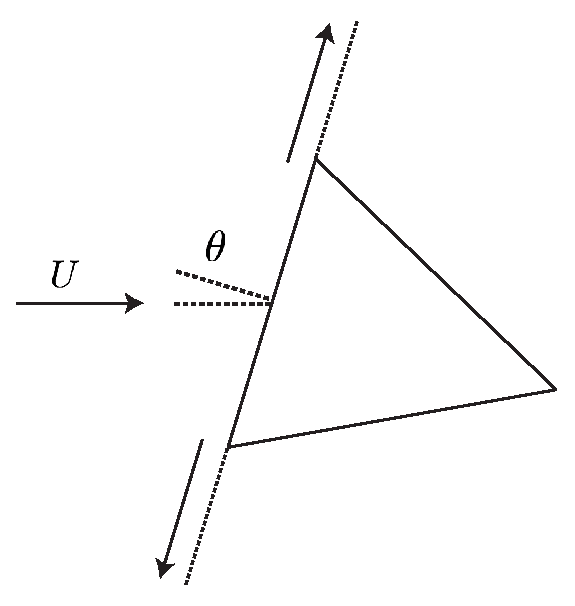
\includegraphics[width=0.25\unitlength]{./chapter-cross-sections/fnp/tri-sketch.eps}}         
      
      
   
 	\put(0.38,0.937){$\theta$}
 	%\put(0.52,0.74){$l$}
   

 	
 	 

     

  \end{picture}

 \caption{Illustration of the lines along which the flow velocity magnitudes have been extracted. The data have been extracted along a line starting from the separation points in the outward direction (shown with arrows) for the top and bottom surfaces.}
    \label{fig:tri-sketch}
\end{figure}


\begin{figure}
  \setlength{\unitlength}{\textwidth}

        \begin{picture}(1,1.1)(0,0.35)

      % % % Parkinson Data 
      \put(0.1,1.1){\includegraphics[width=0.75\unitlength]{./chapter-cross-sections/fnp/vel_prof-tri-4.eps}}
      \put(0.1,0.737){\includegraphics[width=0.75\unitlength]{./chapter-cross-sections/fnp/vel_prof-tri-16.eps}}
      \put(0.1,0.38){\includegraphics[width=0.75\unitlength]{./chapter-cross-sections/fnp/vel_prof-tri-21.eps}}
     
      
      



%      
    \put(0.21,1.41){\small(a)}
     \put(0.21,1.05){\small(b)}
     \put(0.21,0.69){\small(c)}
\put(0.1,0.95){$\displaystyle V_m$}
\put(0.1,1.3){$\displaystyle V_m$}
\put(0.1,0.56){$\displaystyle V_m$}
\put(0.34,0.35){Distance from the leading edge}

      
    \end{picture}

    \caption{Velocity magnitudes of the flow along a line parallel to the front surface spreading towards top (\solidrule) and bottom (\dashedrule) boundaries (figure \ref{fig:tri-sketch}). These two lines (for the top and bottom surfaces) start from the top and bottom leading edges of the triangular cross section. Data present (a) $\alpha=4^\circ$, (b) $\alpha=16^\circ$ \ and (c) $\alpha=21^\circ$.}
    \label{fig:surf_pres}
\end{figure}

 %vspace{10cm}



The maximum velocity magnitude in the top wall jet at $\theta= 4^{\circ}$ (figure \ref{fig:vel-profile} (a)) is higher than that in the corresponding bottom wall jet, leading to a lower pressure at the top edge. However, the velocity magnitude in the bottom wall jet becomes greater than that in the top wall jet at $\theta=16^{\circ}$. The difference between the top and bottom velocity magnitude in these wall jets tends to increase as $\theta$ is increased to $21^{\circ}$, where the velocity magnitude at the bottom is greater than at the top (figure \ref{fig:vel-profile} (c)). This effectively creates the pressure difference (according to the Bernoulli's principle ) shown in figure \ref{fig:surf_pres} (c), which leads to a positive \cy\ and results in a forcing which is in phase with the velocity of the body. 






\subsection{Mean streamlines}
\label{sec:streamlines}

The magnitude of the strain rate tensor is an excellent way of the visualising the shear layers as the strain rate is directly proportional to the shear stress and hence, will be high in the shear layers. The instantaneous flow-field data consists of vortex shedding on top of the shear layers. Therefore, the flow-field data are time averaged over a vortex shedding cycle to filter out the vortex shedding . 

The strain rate tensor of the flow can be expressed as,

\begin{equation}
\varphi = \frac{1}{2}
\begin{bmatrix}
2\frac{\partial u}{\partial x} & \frac{\partial u}{\partial y} + \frac{\partial v}{\partial x} \\
\frac{\partial v}{\partial x} + \frac{\partial u}{\partial y} & 2\frac{\partial v}{\partial y} \\
\end{bmatrix}
\end{equation}

thus the magnitude of the strain rate tensor becomes,
%
\begin{equation}
|\varphi| = \frac{1}{2}\left(4\frac{\partial u}{\partial x}\frac{\partial v}{\partial y} + \left(\frac{\partial u}{\partial y} + \frac{\partial v}{\partial x}\right)^2\right)
\end{equation}.


\begin{figure}[!h]

  \setlength{\unitlength}{\textwidth}

  \begin{picture}(1,0.35)(0,0.725)

    \put(-0.01,0.76){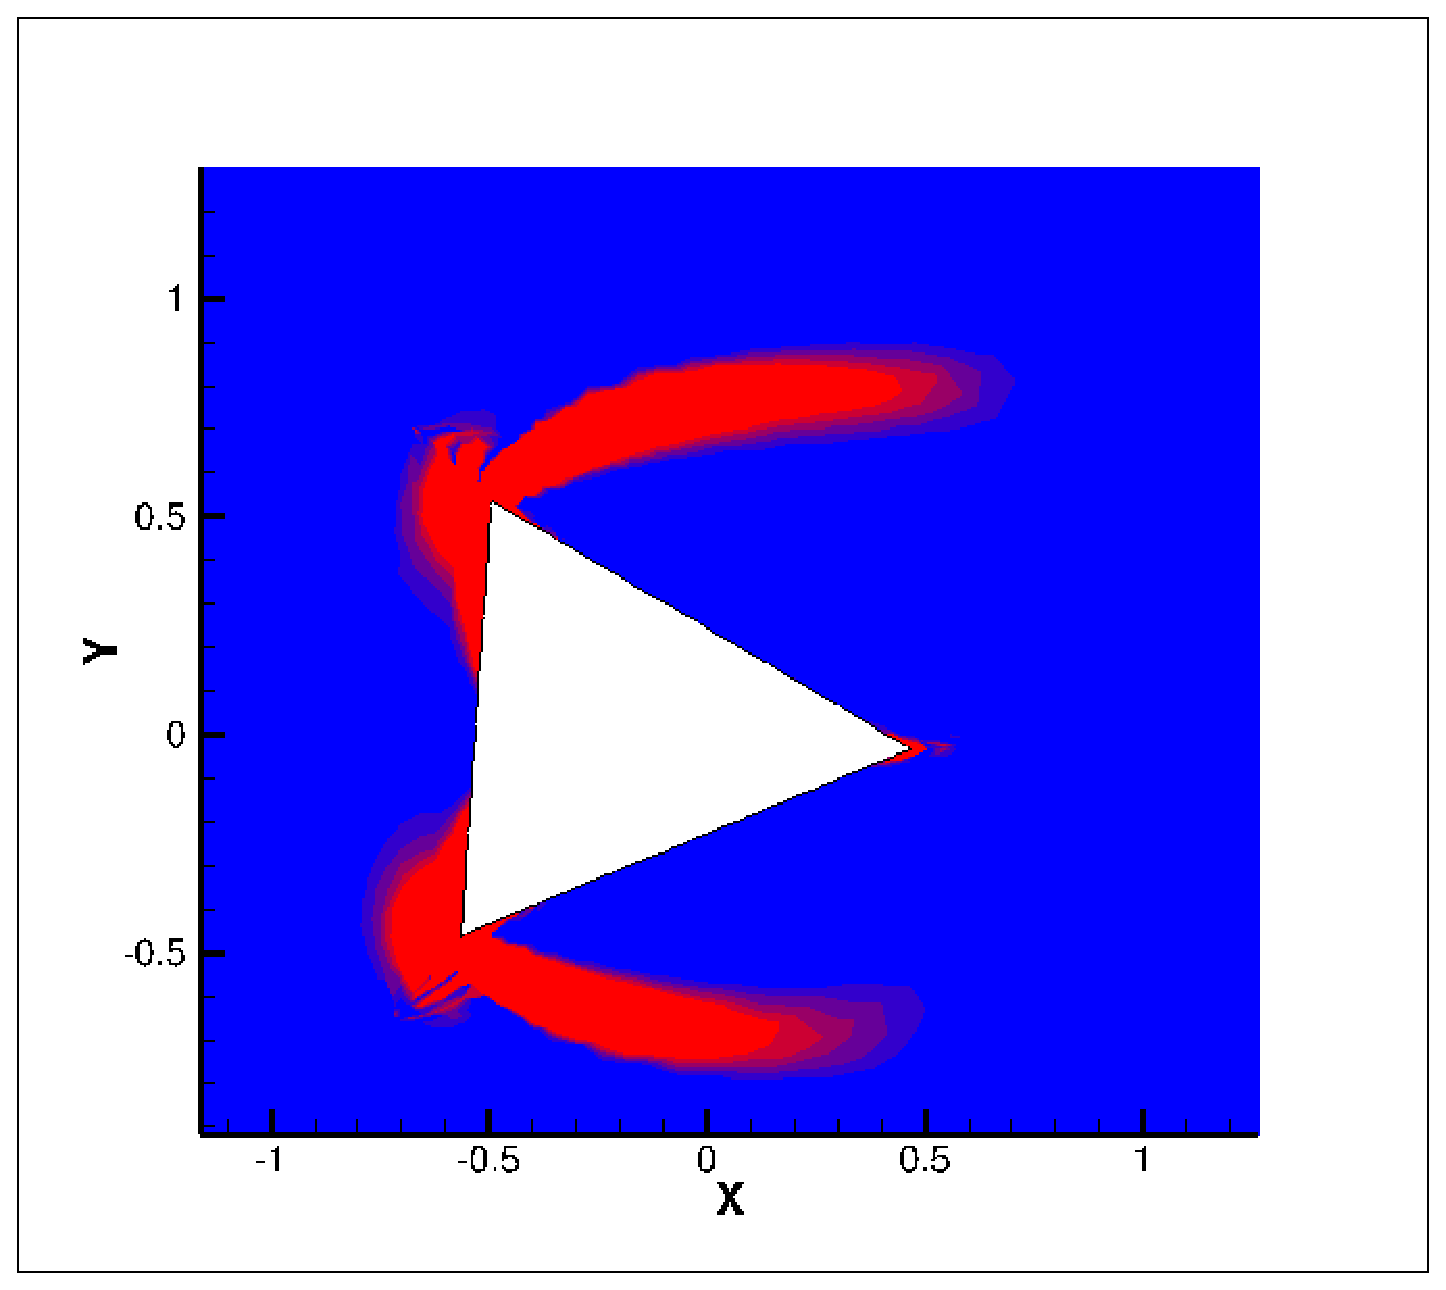
\includegraphics[width=0.33\unitlength]{./chapter-cross-sections/fnp/4.eps}}
    \put(0.335,0.76){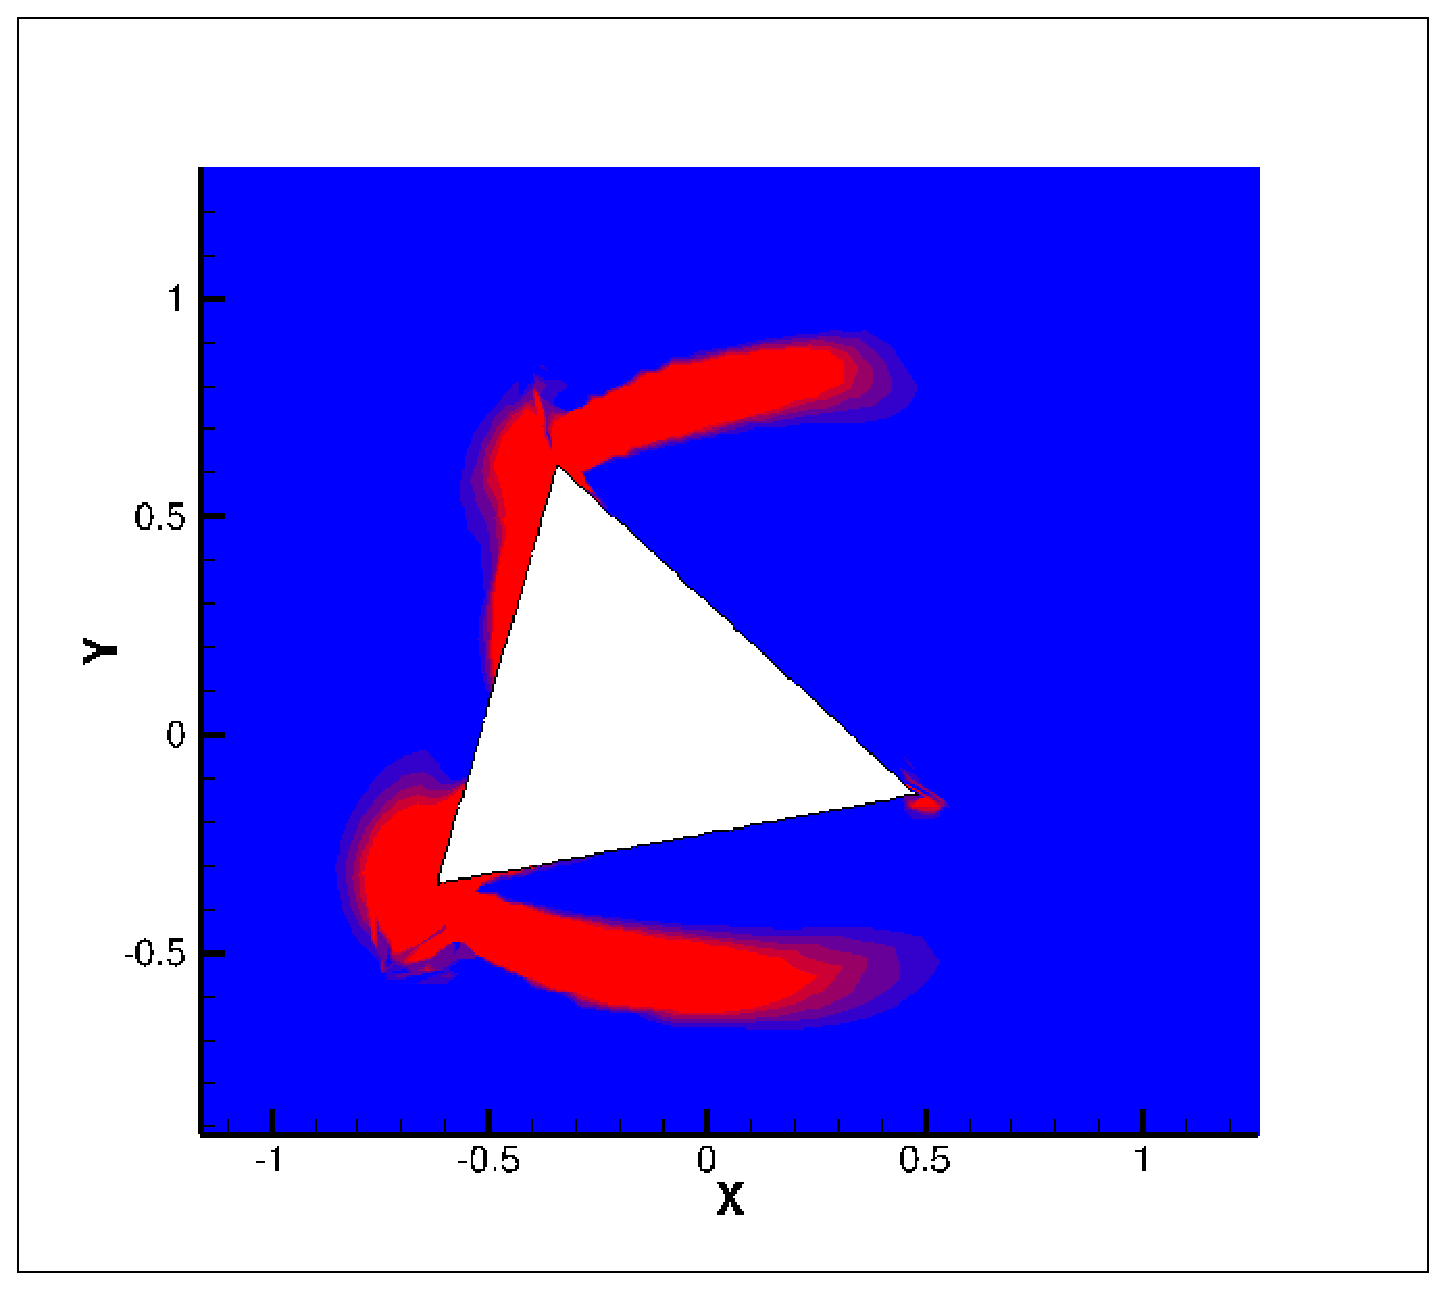
\includegraphics[width=0.33\unitlength]{./chapter-cross-sections/fnp/16.eps}}
    \put(0.68,0.76){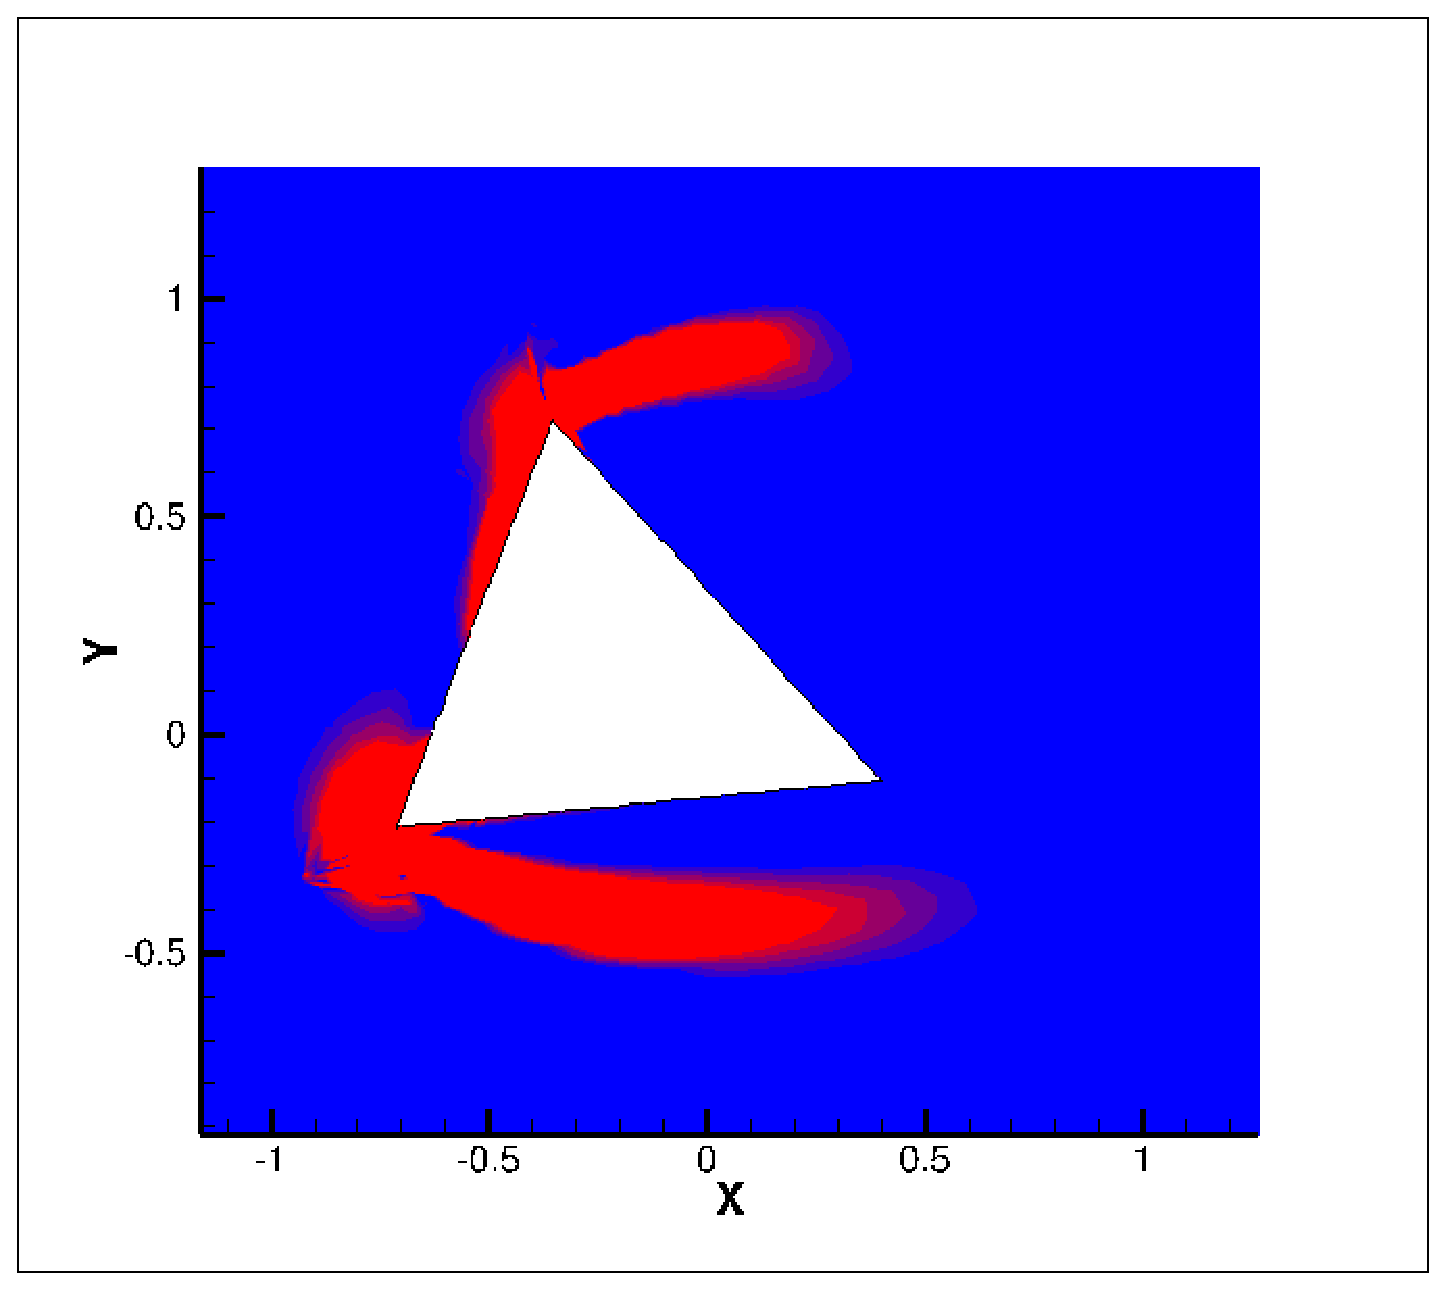
\includegraphics[width=0.33\unitlength]{./chapter-cross-sections/fnp/21.eps}}

   
    
    \put(0.0,0.735){(a)}    
    \put(0.34,0.735){(b)}
    \put(0.685,0.735){(c)}
  
  \end{picture}

  \caption{Contours of the magnitude of the shear strain rate of time averaged flow field on the  stationary isosceles triangle ($\ratio=0$) at $\reynoldsnumber=200$ at different incidence angles. (a) $4^{\circ}$ ( negative value of \cy\ that is further decreasing with increasing $\theta$), (b) $16^{\circ}$ ( negative value of \cy\ that is increasing with increasing $\theta$) and (c) $21^{\circ}$ (a significantly positive value of \cy). The bottom shear layer comes closer to the bottom wall and as the angle of incidence increases.}
  \label{fig:triangle-shear_layers}
\end{figure}




  


Contours of the magnitude of the strain rate tensor of the time-averaged flow-fields of the stationary isosceles triangle are presented in figure \ref{fig:triangle-shear_layers}. Data present at $\theta=4^{\circ}$, $\theta=16^{\circ}$ and $\theta=21^{\circ}$. It can be observed that the proximity of the bottom shear layer increases as $\theta$ is increased from $4^{\circ}-21^{\circ}$. 
%

Through a comparison of the pressure and velocity plot together with the flow-field data, it is clearly evident that two mechanisms govern the transverse forcing. 


%By comparing the pressure and the velocity plots together with the flow-field data, it is evident that there are two mechanisms governing the transverse forcing. The first mechanism is the pressure difference in each shear layer, created as a result of the uneven distribution of the flow created due to the profile and  positioning (angle of attack) of the geometry. This uneven distribution creates a different speed wall jet on either side, and a simple consideration of Bernoulli's equation suggests the higher speed jet will have a lower pressure. This forcing occur out of phase or in the opposite direction of the transverse velocity of the body, as the lower speed (higher pressure) jet is formed on the lower side of the body (when the body is travelling down). The second mechanism is the relative proximity of the top and bottom shear layers. Regardless of the pressure in each shear layer, that pressure will have a larger influence on the force on the body the closer the shear layer is to the body. So, there are two ways to manipulate the force from the shear layers; increase the pressure difference between the shear layers by increasing the difference between the flow in each shear layer (a ``streaming effect''); move the shear layers closer or further from the body (the ``proximity effect'').
%
%Initially at $\theta= 4^{\circ}$ the streaming effect dominates. This can be observed comparing figures \ref{fig:triangle-shear_layers} (a) to (b) and (c). The  bottom shear layer is far from the body at $\theta= 4^{\circ}$, hence the proximity effect is low. This results in the negative \cy.   
%
%As $\theta$ is increased first to $\theta=16^{\circ}$ and then to $21^{\circ}$, the proximity of the bottom shear layer to the wall of the body increases (figure \ref{fig:triangle-shear_layers} (b) and (c)), and thus the proximity effect becomes more dominant. At least for the $\theta = 21^{\circ}$ case, this creates the positive region of the \cy\ vs. $\theta$ curve. 
% 
 
 \begin{figure}[!h]

  \setlength{\unitlength}{\textwidth}

  \begin{picture}(1,0.35)(0,0.725)

    \put(-0.01,0.76){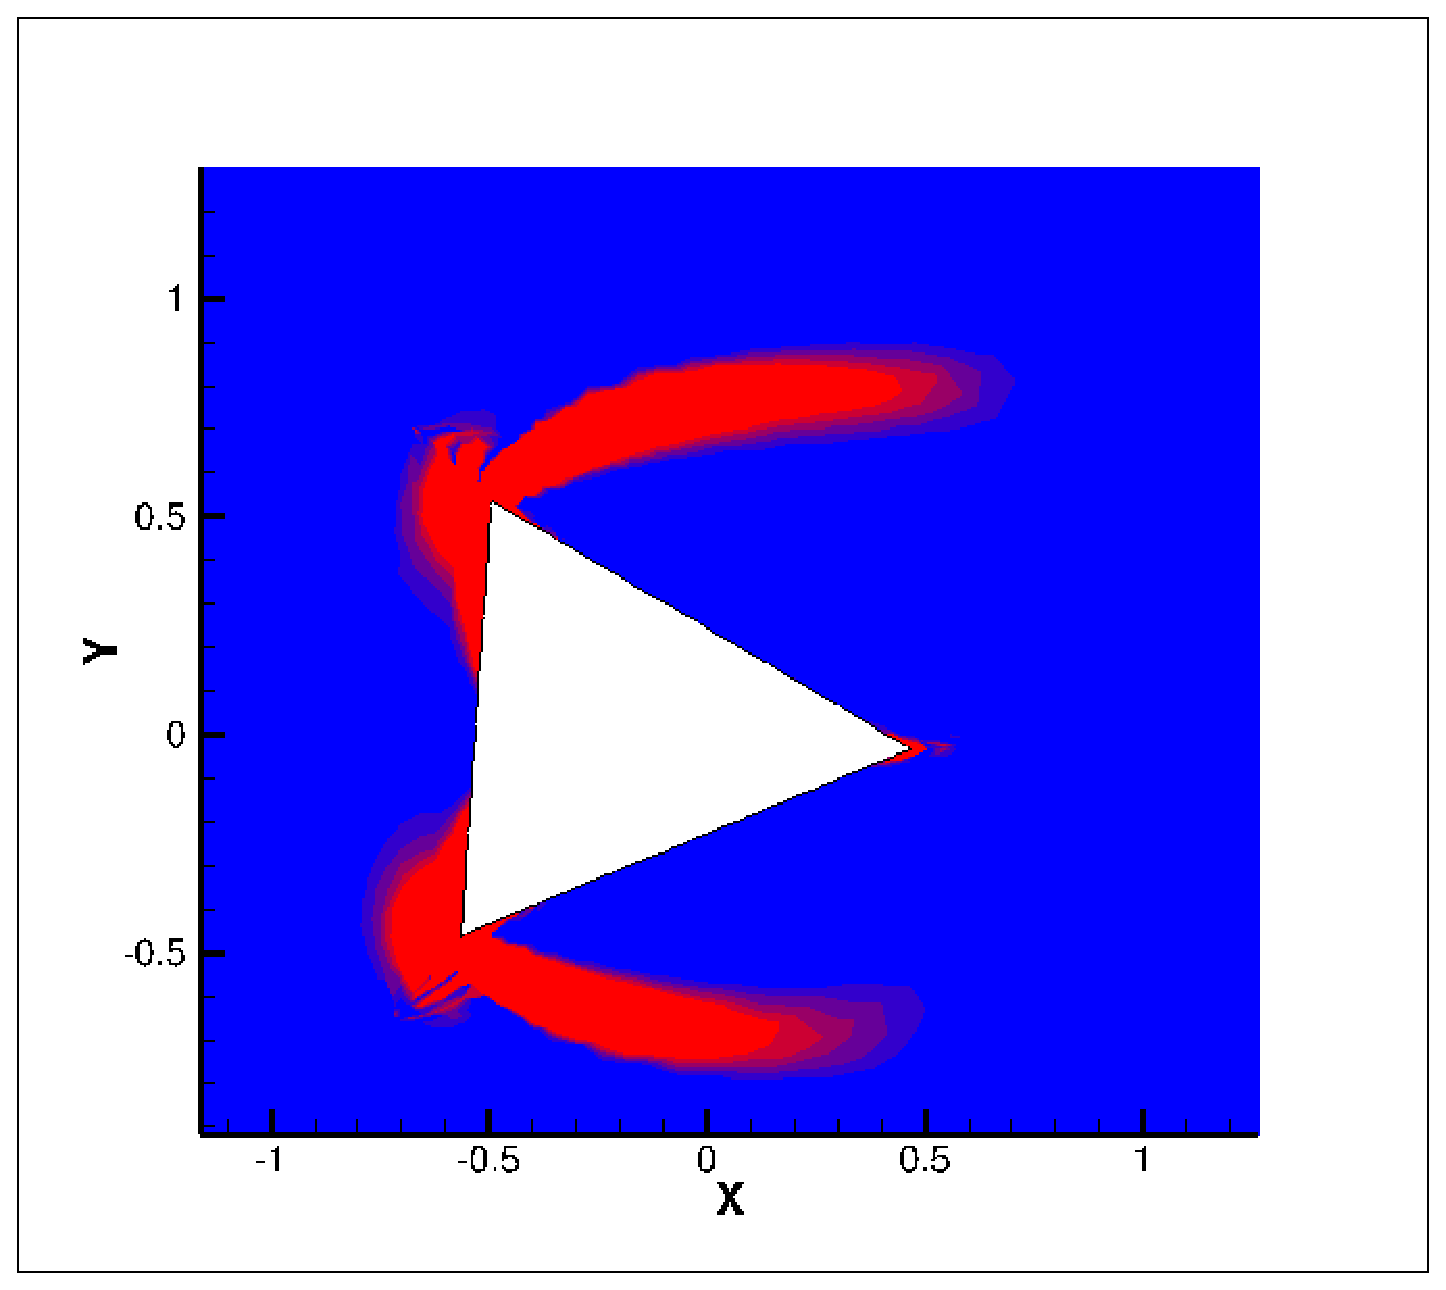
\includegraphics[width=0.33\unitlength]{./chapter-cross-sections/fnp/4.eps}}
    \put(0.335,0.76){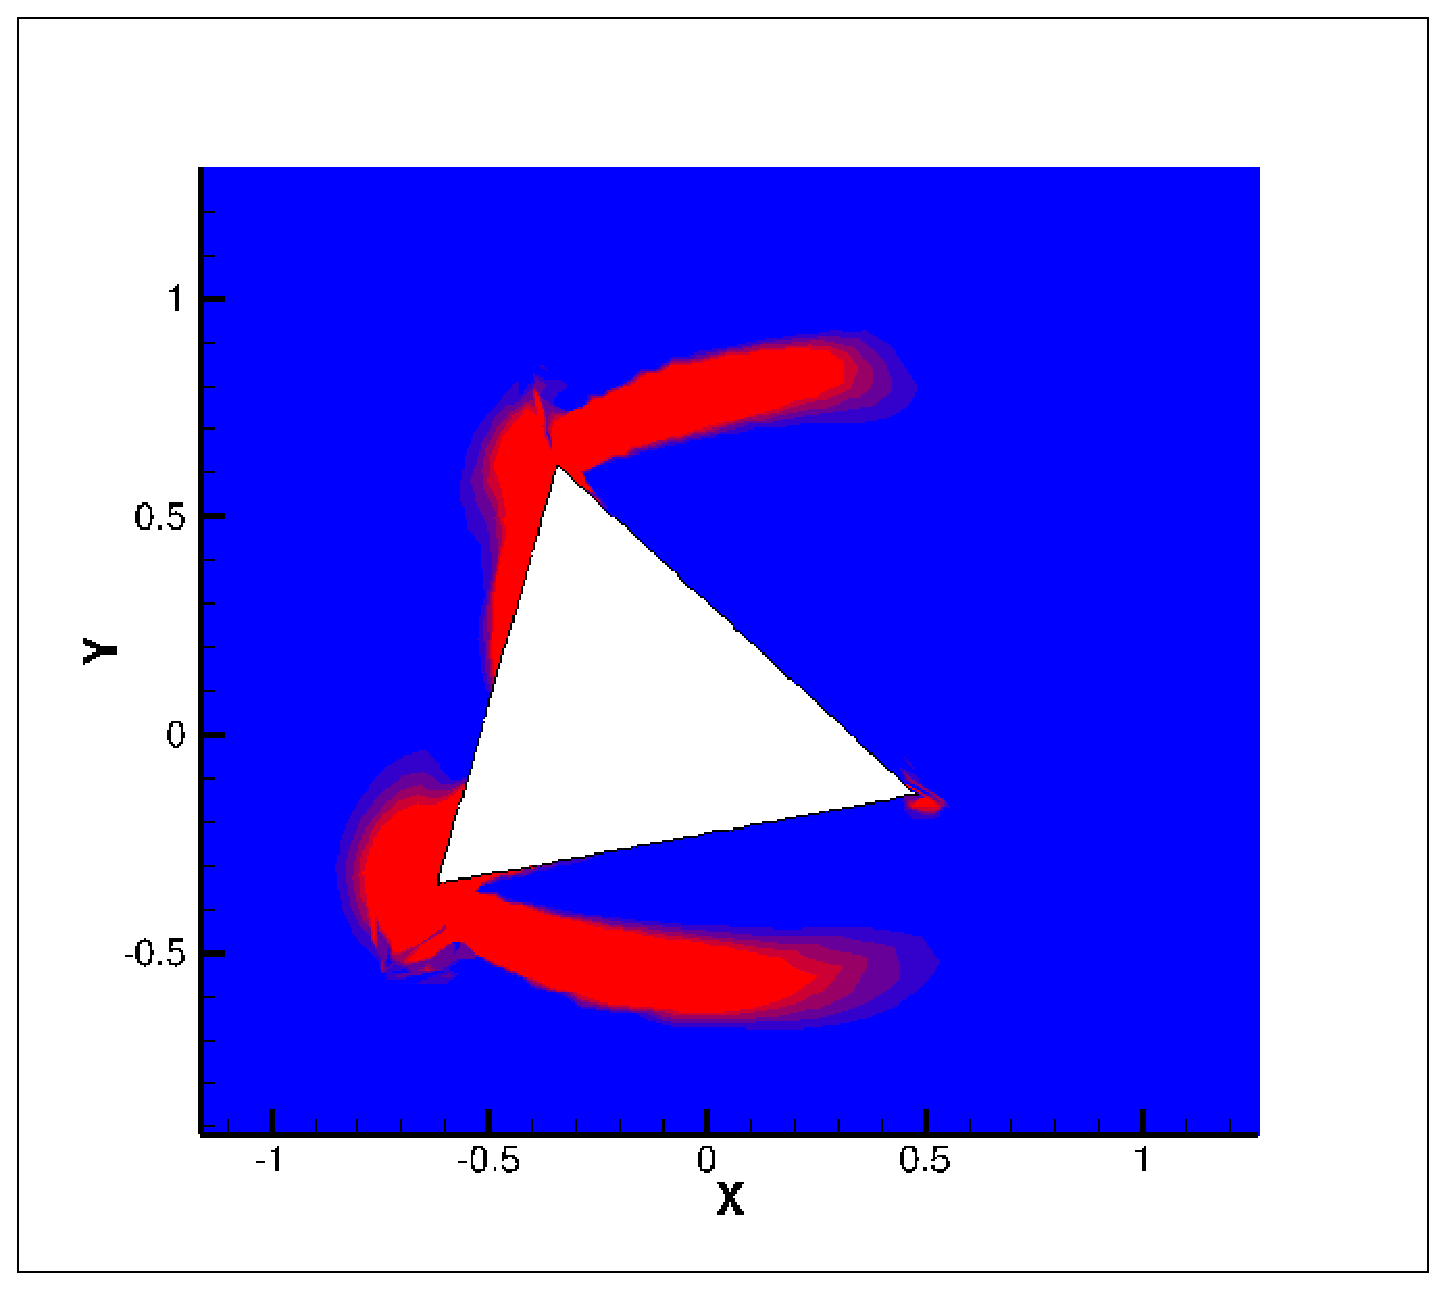
\includegraphics[width=0.33\unitlength]{./chapter-cross-sections/fnp/16.eps}}
    \put(0.68,0.76){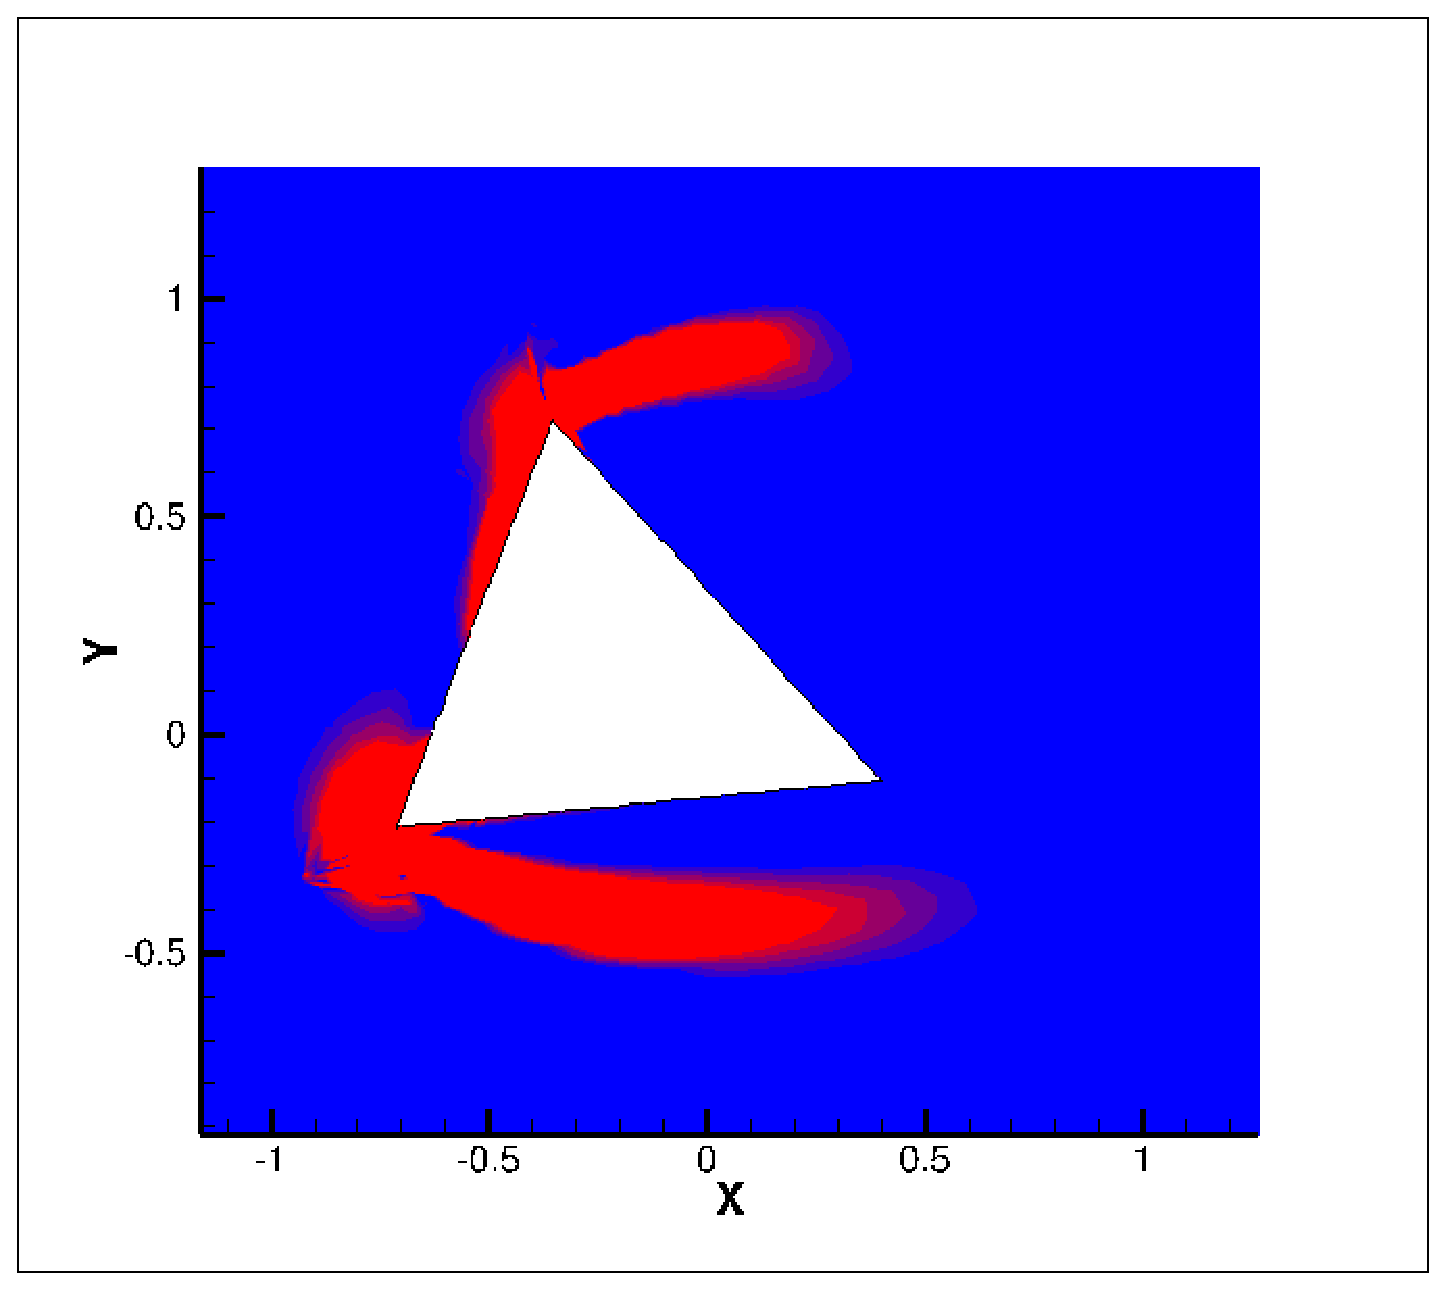
\includegraphics[width=0.33\unitlength]{./chapter-cross-sections/fnp/21.eps}}

   
    
    \put(0.0,0.735){(a)}    
    \put(0.34,0.735){(b)}
    \put(0.685,0.735){(c)}
  
  \end{picture}

  \caption{Contours of the magnitude of the shear strain rate of time averaged flow field on the  stationary isosceles triangle ($\ratio=0$) at $\reynoldsnumber=200$ at different incidence angles. (a) $4^{\circ}$ ( negative value of \cy\ that is further decreasing with increasing $\theta$), (b) $16^{\circ}$ ( negative value of \cy\ that is increasing with increasing $\theta$) and (c) $21^{\circ}$ (a significantly positive value of \cy). The bottom shear layer comes closer to the bottom wall and as the angle of incidence increases.}
  \label{fig:triangle-shear_layers}
\end{figure}




  

 
 % !TeX spellcheck = en_GB
\begin{figure}[!htb]
  \setlength{\unitlength}{\textwidth}

        \begin{picture}(1,0.4)(-0.02,0)

 
      
      \put(0.08,0.02){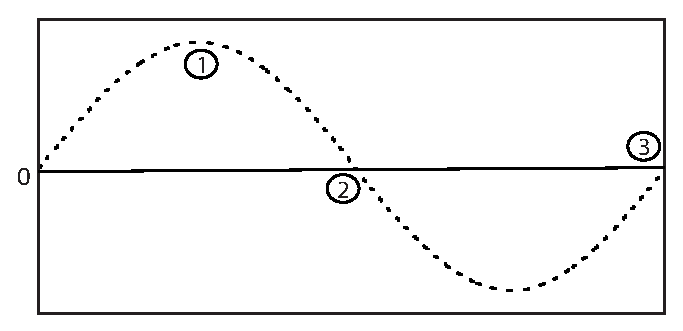
\includegraphics[width=0.75\unitlength]{./chapter-cross-sections/fnp/fsi_flow_sketch.eps}}

      %\put(0.46,0.00){\massdamp}
      
      
     
       %\put(0.03,0.235){$\displaystyle\frac{P_{m}}{\rho \mathcal{A}U^3 }$}
      

      %\put(0.095,0.218){\small(a)}
      %\put(0.565,0.218){\small(b)}
      
    \end{picture}

  \caption{}
    \label{fig:power_curves}
\end{figure}

 %vspace{10cm}

 
 
 \begin{figure}[htbp]
  \setlength{\unitlength}{\textwidth}

  \begin{picture}(1,1.19)(0,0)
    % % %90
      % % % Parkinson Data 
      \put(0.005,0.8){\includegraphics[width=0.4\unitlength]{./chapter-cross-sections/fnp/{fsi-0.25-1}.eps}}
      \put(0.005,0.4){\includegraphics[width=0.4\unitlength]{./chapter-cross-sections/fnp/{fsi-0.25-2}.eps}}
      \put(0.005,0.0){\includegraphics[width=0.4\unitlength]{./chapter-cross-sections/fnp/{fsi-0.25-3}.eps}}

      
      
      \put(0.505,0.8){\includegraphics[width=0.4\unitlength]{./chapter-cross-sections/fnp/{qss-0.25-1}.eps}}
      \put(0.505,0.4){\includegraphics[width=0.4\unitlength]{./chapter-cross-sections/fnp/{qss-0.25-3}.eps}}
      \put(0.505,0.0){\includegraphics[width=0.4\unitlength]{./chapter-cross-sections/fnp/{qss-0.25-3}.eps}} 
      
      
%      \put(0.23,0.00){ $\displaystyle\frac{c}{\rho\mathcal{A}U}$}
%      \put(0.73,0.00){ $\displaystyle\frac{c}{\rho\mathcal{A}U}$}


      
      \put(0.01,1.125){\small(a)}
      \put(0.510,1.125){\small(b)}
      \put(0.01,0.725){\small(c)}
      \put(0.510,0.725){\small(d)}
      \put(0.01,0.33){\small(e)}
      \put(0.510,0.33){\small(f)}
      
   
   
      

  \end{picture}

  \caption{Time averaged stream functions of stationary and oscillating flow-fields of the hybrid cross section ($\ratio=0.25$), averaged over a vortex shedding cycle. (a), (c) and (e) are the averaged stream functions of the oscillating case at $\frac{tU}{D}=2295.763$ (point 1), $\frac{tU}{D}=2305.897$ (point 2) and $\frac{tU}{D}=2325.870$ (point 3) . (b), (d) and (f) are the stream functions of the flow field of the stationary body corresponding to the induced angles of (a), (c) and (e).}  
  \label{fig:flow_field_FSI}
\end{figure}
 
 